%%%%%%%%%%%%%%%%%%%%%%%%%%%%%%%%%%%%%%%%%%%%%%%%%%%%%%%%%%%%%%%%%%%%%%%%%%%%%%%%%%%%
% Template for STAT 547C final project
% Author: Ben Bloem-Reddy <benbr@stat.ubc.ca>
% Date: Oct. 18, 2019
%%%%%%%%%%%%%%%%%%%%%%%%%%%%%%%%%%%%%%%%%%%%%%%%%%%%%%%%%%%%%%%%%%%%%%%%%%%%%%%%%%%%

% Note: You will get an empty bibliography warning when compiling until you include a citation.
\documentclass[10pt]{article}
\usepackage{lipsum} 
\usepackage{graphicx} 
\usepackage{environ} 
\usepackage[left=3.5cm, right=3.5cm]{geometry}
% header.tex
% this is where you load pacakges, specify custom formats, etc.

\usepackage[left=1in,right=1in,top=0.75in,footskip=25pt]{geometry} 
% \usepackage{changepage}
\usepackage{amsmath,amsthm,amssymb,amsfonts}
\usepackage{mathtools}
% enumitem for custom lists
\usepackage{enumitem}
% Load dsfont this to get proper indicator function (bold 1) with \mathds{1}:
\usepackage{dsfont}
\usepackage{centernot}

\usepackage[usenames,dvipsnames]{xcolor}

% set up commenting code (I will use this during marking)
\definecolor{CommentColor}{rgb}{0,.50,.50}
\newcounter{margincounter}
\newcommand{\displaycounter}{{\arabic{margincounter}}}
\newcommand{\incdisplaycounter}{{\stepcounter{margincounter}\arabic{margincounter}}}
\newcommand{\COMMENT}[1]{\textcolor{CommentColor}{$\,^{(\incdisplaycounter)}$}\marginpar{\scriptsize\textcolor{CommentColor}{ {\tiny $(\displaycounter)$} #1}}}

\usepackage{appendix}

% set up graphics
\usepackage{graphicx}
\DeclareGraphicsExtensions{.pdf,.png,.jpg}
\graphicspath{ {fig/} }

\usepackage[sorting=nyt,backend=biber,bibstyle=alphabetic,citestyle=alphabetic,giveninits=true]{biblatex}

\usepackage{fancyhdr}
\pagestyle{fancy}
\setlength{\headheight}{40pt}

%%%%%%%%%%%%%%%%%%%%%%%%%%%%%%%%%%%%%%%%%%%%%%%%%%%%%%%%%%%%%%%%%%%%%%%%%%%%%%%%%%%%
% most other packages you might use should be loaded before hyperref
%%%%%%%%%%%%%%%%%%%%%%%%%%%%%%%%%%%%%%%%%%%%%%%%%%%%%%%%%%%%%%%%%%%%%%%%%%%%%%%%%%%%

% Set up hyperlinks:
\definecolor{RefColor}{rgb}{0,0,.65}
\usepackage[colorlinks,linkcolor=RefColor,citecolor=RefColor,urlcolor=RefColor]{hyperref}

\usepackage[capitalize]{cleveref}
\crefname{appsec}{Appendix}{Appendices} % you can tell cleveref what to call things
% defs.tex
% this is where you define custom notation, commands, etc.


%%
% full alphabets of different styles
%%

% bf series
\def\bfA{\mathbf{A}}
\def\bfB{\mathbf{B}}
\def\bfC{\mathbf{C}}
\def\bfD{\mathbf{D}}
\def\bfE{\mathbf{E}}
\def\bfF{\mathbf{F}}
\def\bfG{\mathbf{G}}
\def\bfH{\mathbf{H}}
\def\bfI{\mathbf{I}}
\def\bfJ{\mathbf{J}}
\def\bfK{\mathbf{K}}
\def\bfL{\mathbf{L}}
\def\bfM{\mathbf{M}}
\def\bfN{\mathbf{N}}
\def\bfO{\mathbf{O}}
\def\bfP{\mathbf{P}}
\def\bfQ{\mathbf{Q}}
\def\bfR{\mathbf{R}}
\def\bfS{\mathbf{S}}
\def\bfT{\mathbf{T}}
\def\bfU{\mathbf{U}}
\def\bfV{\mathbf{V}}
\def\bfW{\mathbf{W}}
\def\bfX{\mathbf{X}}
\def\bfY{\mathbf{Y}}
\def\bfZ{\mathbf{Z}}

% bb series
\def\bbA{\mathbb{A}}
\def\bbB{\mathbb{B}}
\def\bbC{\mathbb{C}}
\def\bbD{\mathbb{D}}
\def\bbE{\mathbb{E}}
\def\bbF{\mathbb{F}}
\def\bbG{\mathbb{G}}
\def\bbH{\mathbb{H}}
\def\bbI{\mathbb{I}}
\def\bbJ{\mathbb{J}}
\def\bbK{\mathbb{K}}
\def\bbL{\mathbb{L}}
\def\bbM{\mathbb{M}}
\def\bbN{\mathbb{N}}
\def\bbO{\mathbb{O}}
\def\bbP{\mathbb{P}}
\def\bbQ{\mathbb{Q}}
\def\bbR{\mathbb{R}}
\def\bbS{\mathbb{S}}
\def\bbT{\mathbb{T}}
\def\bbU{\mathbb{U}}
\def\bbV{\mathbb{V}}
\def\bbW{\mathbb{W}}
\def\bbX{\mathbb{X}}
\def\bbY{\mathbb{Y}}
\def\bbZ{\mathbb{Z}}

% cal series
\def\calA{\mathcal{A}}
\def\calB{\mathcal{B}}
\def\calC{\mathcal{C}}
\def\calD{\mathcal{D}}
\def\calE{\mathcal{E}}
\def\calF{\mathcal{F}}
\def\calG{\mathcal{G}}
\def\calH{\mathcal{H}}
\def\calI{\mathcal{I}}
\def\calJ{\mathcal{J}}
\def\calK{\mathcal{K}}
\def\calL{\mathcal{L}}
\def\calM{\mathcal{M}}
\def\calN{\mathcal{N}}
\def\calO{\mathcal{O}}
\def\calP{\mathcal{P}}
\def\calQ{\mathcal{Q}}
\def\calR{\mathcal{R}}
\def\calS{\mathcal{S}}
\def\calT{\mathcal{T}}
\def\calU{\mathcal{U}}
\def\calV{\mathcal{V}}
\def\calW{\mathcal{W}}
\def\calX{\mathcal{X}}
\def\calY{\mathcal{Y}}
\def\calZ{\mathcal{Z}}


%%%%%%%%%%%%%%%%%%%%%%%%%%%%%%%%%%%%%%%%%%%%%%%%%%%%%%%%%%
% text short-cuts
\def\iid{i.i.d.\ } %i.i.d.
\def\ie{i.e.\ }
\def\eg{e.g.\ }
\def\Polya{P\'{o}lya\ }
%%%%%%%%%%%%%%%%%%%%%%%%%%%%%%%%%%%%%%%%%%%%%%%%%%%%%%%%%%

%%%%%%%%%%%%%%%%%%%%%%%%%%%%%%%%%%%%%%%%%%%%%%%%%%%%%%%%%%
% quasi-universal probabilistic and mathematical notation
% my preferences (modulo publication conventions, and clashes like random vectors):
%   vectors: bold, lowercase
%   matrices: bold, uppercase
%   operators: blackboard (e.g., \mathbb{E}), uppercase
%   sets, spaces: calligraphic, uppercase
%   random variables: normal font, uppercase
%   deterministic quantities: normal font, lowercase
%%%%%%%%%%%%%%%%%%%%%%%%%%%%%%%%%%%%%%%%%%%%%%%%%%%%%%%%%%

% operators
\def\P{\bbP} %fundamental probability
\def\E{\bbE} %expectation
% conditional expectation
\DeclarePairedDelimiterX\bigCond[2]{[}{]}{#1 \;\delimsize\vert\; #2}
\newcommand{\conditional}[3][]{\bbE_{#1}\bigCond*{#2}{#3}}
\def\Law{\mathcal{L}} %law; this is by convention in the literature
\def\indicator{\mathds{1}} % indicator function

% sets and groups
\def\borel{\calB} %Borel sets
\def\sigAlg{\calA} %sigma-algebra
\def\filtration{\calF} %filtration
\def\grp{\calG} %group

% binary relations
\def\condind{{\perp\!\!\!\perp}} %independence/conditional independence
\def\equdist{\stackrel{\text{\rm\tiny d}}{=}} %equal in distribution
\def\equas{\stackrel{\text{\rm\tiny a.s.}}{=}} %euqal amost surely
\def\simiid{\sim_{\mbox{\tiny iid}}} %sampled i.i.d

% common vectors and matrices
\def\onevec{\mathbf{1}}
\def\iden{\mathbf{I}} % identity matrix
\def\supp{\text{\rm supp}}

% misc
% floor and ceiling
\DeclarePairedDelimiter{\ceilpair}{\lceil}{\rceil}
\DeclarePairedDelimiter{\floor}{\lfloor}{\rfloor}
\newcommand{\argdot}{{\,\vcenter{\hbox{\tiny$\bullet$}}\,}} %generic argument dot
%%%%%%%%%%%%%%%%%%%%%%%%%%%%%%%%%%%%%%%%%%%%%%%%%%%%%%%%%%

%%%%%%%%%%%%%%%%%%%%%%%%%%%%%%%%%%%%%%%%%%%%%%%%%%%%%%%%%%
%% some distributions
% continuous
\def\UnifDist{\text{\rm Unif}}
\def\BetaDist{\text{\rm Beta}}
\def\ExpDist{\text{\rm Exp}}
\def\GammaDist{\text{\rm Gamma}}
% \def\GenGammaDist{\text{\rm GGa}} %Generalized Gamma

% discrete
\def\BernDist{\text{\rm Bernoulli}}
\def\BinomDist{\text{\rm Binomial}}
\def\PoissonPlus{\text{\rm Poisson}_{+}}
\def\PoissonDist{\text{\rm Poisson}}
\def\NBPlus{\text{\rm NB}_{+}}
\def\NBDist{\text{\rm NB}}
\def\GeomDist{\text{\rm Geom}}
% \def\CRP{\text{\rm CRP}}
% \def\EGP{\text{\rm EGP}}
% \def\MittagLeffler{\text{\rm ML}}
%%%%%%%%%%%%%%%%%%%%%%%%%%%%%%%%%%%%%%%%%%%%%%%%%%%%%%%%%%

%%%%%%%%%%%%%%%%%%%%%%%%%%%%%%%%%%%%%%%%%%%%%%%%%%%%%%%%%%
% Project-specific notation should go here
% (Because it's at the end of the file, it can overwrite anything that came before.)

%e.g.,
\def\Laplacian{\calL}
\def\P{\calP}

% combinatorial objects
\def\perm{\sigma} %fixed permutation
\def\Perm{\Sigma} %random permutation
\def\part{\pi} %fixed partition
\def\Part{\Pi} %random partition


%%%%%%%%%%%%%%%%%%%%%%%%%%%%%%%%%%%%%%%%%%%%%%%%%%%%%%%%%%
\newtheorem{definition}{Definition}
\newtheorem{theorem}{Theorem}
\newtheorem{example}{Example}

\newcommand\numberthis{\addtocounter{equation}{1}\tag{\theequation}}

\usepackage[style=apa, backend=biber]{biblatex}
\addbibresource{main.bib}
\nocite{*}

%%%%%%%%%%%%%%%%%%%%%%%%%%%%%%%%%%%%%%%%%%%%%%%%%%%%%%%%%%%%%%%%%%%%%%%%%%%%%%%%%

% your title/author/date information go here
\title{An Introduction to Probabalistic Programming with Markov Chain Monte Carlo (MCMC)} % replace with your title
\author{Daniel Polson} % replace with your name
\date{12/15/2022} % replace with your submission date

% start of document
\begin{document}

\NewEnviron{NSMALL}{
    \scalebox{1}{$\BODY$} 
} 

\maketitle


\section{Background}

Markov Chain Monte Carlo (MCMC) is a class of algorithms for sampling from a probability distribution. The idea behind MCMC is to construct a Markov chain that has the desired distribution as its equilibrium distribution, and then to sample from the chain after it has reached equilibrium. This allows us to draw samples from a distribution without having to directly compute the distribution. The methods focussed on in this paper include the Metropolis-Hastings Algorithm \cite{hast}, and the Gibbs Sampler \cite{gibbs}. These are long-used variations of MCMC, and continue to be in use to this day. The paper below requires some prior knowledge of measure theory and probability theory to prove the usefulness of these methods, and follows up with some basic applications.


\section{Metropolis-Hastings Algorithm}

%Define stationary distributions

\subsection{Theory}

\begin{definition}
    Let $\left( E, \calE \right)$ be a measurable space. A transition interval from $\left( E, \calE \right)$ into $\left( E, \calE \right)$ is considered a Markov Kernel whenever $K \left( x, E \right) = 1$ for all $x$.
\end{definition}


%%Fubinis Theorem

\begin{definition}
    A Markov Kernel $K \left( x, A \right)$ is called reversible with respect to $\pi$ if for all bounded measurable functions $f$ from $X \times X$ to $\bbR$, 
    \begin{align*}
        \int \int _{X \times X} f \left( x, y \right) \pi \left( dx \right) K \left( x, dy \right) &= \int \int _{X \times X} f \left( y, x \right) \pi \left( dx \right) K \left( x, dy \right).
    \end{align*}
\end{definition}

\begin{definition}
    The probability measure $\pi$ is called invariant for a function $P$ whenever $\pi = \pi P$, and $\pi$ is called the stationary distribution of $P$.
\end{definition}
\noindent
Before defining the Metropolis-Hastings update, we require some prior notation. Let $g$ be the unnormalized density function with respect to a positive measure $\mu$, and let $q \left( x, \cdot \right)$ be a normalized density function with respect to $\mu$. Define:
\begin{align*}
    r \left( x, y \right) &= \frac{g \left( y \right) q \left( y, x \right)}{g \left( x \right) q \left( x, y \right)}
\end{align*}
And,
\begin{align*}
    a \left( x, y \right) &= \text{min} \left( 1, r \left( x, y \right) \right)
\end{align*}

\begin{theorem}
    The Metropolis-Hastings update, which is given as $P_{mh} below$:
    \begin{align*}
        P_{mh} \left( x,A \right) &= \left[ 1 - \int _{A} q \left( x, y \right) a \left( x, y \right) \mu \left( dy \right) \right] \mathbf{1}_{A} \left( x \right) + \int _{A} q \left( x, y \right) a \left( x, y \right) \mu \left( dy \right)
    \end{align*}
    is a Markov kernel.
\end{theorem}
\noindent
\textit{Proof.} 
\begin{align*}
    P_{mh} \left( x,E \right) &= \left[ 1 - \int _{E} q \left( x, y \right) a \left( x, y \right) \mu \left( dy \right) \right] \mathbf{1}_{E} \left( x \right) + \int _{E} q \left( x, y \right) a \left( x, y \right) \mu \left( dy \right) \\[1em]
    &= 1 - \int _{E} q \left( x, y \right) a \left( x, y \right) \mu \left( dy \right) + \int _{E} q \left( x, y \right) a \left( x, y \right) \mu \left( dy \right) \\[1em]
    &= 1 \; \; \; \Box
\end{align*}

\begin{theorem}
    The Metropolis-Hastings update, which is given as $P_{mh}$ below:
    \begin{align*}
        P_{mh} \left( x,A \right) &= \left[ 1 - \int _{A} q \left( x, y \right) a \left( x, y \right) \mu \left( dy \right) \right] \mathbf{1}_{A} \left( x \right) + \int _{A} q \left( x, y \right) a \left( x, y \right) \mu \left( dy \right)
    \end{align*}
    is reversible with respect to the distribution with unnormalized density function $g$.
\end{theorem}

\noindent
\textit{Proof.} Let $\pi$ be the measure with density function $g$ with respect to $\mu$. Then, we have:
\begin{align*}
    \int \int f \left( x, y \right) \pi \left( dx \right) P_{mh} \left( x, dy \right) 
    &= \int \int f \left( x, y \right) g \left( x \right) P_{mh} \left( x, dy \right) \mu \left( dx \right)
\end{align*}
Using the definition of $P_{mh}$, we can update this integral as follows:
\begin{align*}
    \int \int f \left( x, y \right) \pi \left( dx \right) P_{mh} \left( x, dy \right) 
    &= \int \int f \left( x, y \right) g \left( x \right)  \left( 1 - \int _{A} q \left( x, y \right) a \left( x, y \right) \mu \left( dy \right) \right) \mathbf{1}_{dy} \left( x \right) \mu \left( dx \right)  \\[1em]
    &\; \; \; \; \; + \int \int f \left( x, y \right) g \left( x \right) q \left( x, y \right) a \left( x, y \right) \mu \left( dx \right) \mu \left( dy \right) \numberthis \label{eqn}
\end{align*}

\noindent
However, the presence of $\mathbf{1}_{dy} \left( x \right)$ means the second integral in the sum on the right is equal to $0$ wherever $x \neq y$. Thus, we can rewrite this term as:
\begin{align*}
    \int f \left( x, x \right) g \left( x \right)  \left( 1 - \int _{A} q \left( x, y \right) a \left( x, y \right) \mu \left( dy \right) \right) \mu \left( dx \right) 
\end{align*}
But, now the variable we are integrating over becomes arbitrary, so we can rewrite this term once again as:
\begin{align*}
    \int f \left( y, y \right) g \left( y \right)  \left( 1 - \int _{A} q \left( y, x \right) a \left( y, x \right) \mu \left( dx \right) \right) \mu \left( dy \right) 
\end{align*}
Now, consider the second term in the sum on the right-hand side of (1), first considering the case that $r \left( x, y \right) \geq 1$, so that $a \left( x, y \right) = 1$ and $a \left( y, x \right) = r \left( y, x \right)$.
\begin{align*}
    \int \int f \left( x, y \right) g \left( x \right) q \left( x, y \right) a \left( x, y \right) \mu \left( dx \right) \mu \left( dy \right) &= \int \int f \left( x, y \right) g \left( x \right) q \left( x, y \right) \mu \left( dx \right) \mu \left( dy \right) \\[1em]
    &= \int \int f \left( x, y \right) g \left( y \right) q \left( y, x \right) \frac{g \left( x \right) q \left( x, y \right)}{g \left( y \right) q \left( y, x \right)} \mu \left( dx \right) \mu \left( dy \right) \\[1em]
    &= \int \int f \left( x, y \right) g \left( y \right) q \left( y, x \right) a \left( y, x \right) \mu \left( dx \right) \mu \left( dy \right)
\end{align*}
The last equality implies that the order of $x, y$ are irrelevant in this case, so we have:
\begin{align*}
    \int \int f \left( x, y \right) g \left( x \right) q \left( x, y \right) a \left( x, y \right) \mu \left( dx \right) \mu \left( dy \right) &= \int \int f \left( y, x \right) g \left( y \right) q \left( y, x \right) r \left( y, x \right) \mu \left( dx \right) \mu \left( dy \right)
\end{align*}
Therefore, for this case, we find that:
\begin{align*}
    \int \int f \left( x, y \right) \pi \left( dx \right) P_{mh} \left( x, dy \right) &= \int \int f \left( y, x \right) g \left( y \right) q \left( y, x \right) r \left( y, x \right) \mu \left( dx \right) \mu \left( dy \right) \\[1em]
    &\; \; \; \; \; + \int f \left( y, y \right) g \left( y \right)  \left( 1 - \int _{A} q \left( y, x \right) a \left( y, x \right) \mu \left( dx \right) \right) \mu \left( dy \right) 
\end{align*}
Reversing the steps we took in (1) on the right-hand side of the above equation,
\begin{align*}
    \int \int f \left( x, y \right) \pi \left( dx \right) P_{mh} \left( x, dy \right) &= \int \int f \left( y, x \right) \pi \left( dx \right) P_{mh} \left( x, dy \right)
\end{align*}
Thus, the Kernel $P_{mh}$ is reversible with respect to the distribution with unnormalized density function $g$ in this case. The case where $r \left( x, y \right) < 1$ is left as an exercise for the reader.     $\Box$
\\[1\baselineskip]
Now that we have determined the reversibility of $P_{mh}$ with respect to the distribution with unnormalized density function $g$, we find that:
\begin{align*}
    \int \pi \left( dx \right) P_{mh} \left( x, A \right) &= \int \int \mathbf{1}_{A} \left( y \right) \pi \left( dx \right) P_{mh} \left( x, dy \right) \\[1em]
    &= \int \int \mathbf{1}_{A} \left( x \right) \pi \left( dx \right) P_{mh} \left( x, dy \right) \\[1em]
    &= \int \mathbf{1}_{A} \left( x \right) \pi \left( dx \right) \left[ \int P_{mh} \left( x, dy \right)  \right] \\[1em]
    &= \int \mathbf{1}_{A} \left( x \right) \pi \left( dx \right) \\[1em]
    &= \pi \left( A \right)
\end{align*}
\noindent
Where the second equality follows from reversibility, and the second last equality follows from Definition 2. This implies that $\pi = \pi P_{mh}$, meaning that by Definition Y, $\pi$ is invariant for $P_{mh}$, and $\pi$ is the stationary distribution of $P_{mh}$.

\subsection{Application}
\noindent
The above work means that in practice, generating samples using the Metropolis Hastings update will be equivalent to drawing samples from any distribution which we know the unnormalized density function for. The typical usage for this algorithm is to generate samples from a posterior distribution, since the usage of Bayes' Theorem often results in an unnormalized conditional density function. 
\\[1\baselineskip]
\noindent
Bayes' Theorem is difficult to prove in the context of measure theory, but Schervish \cite{schervish} does an excellent job. The basic idea provided is that given a random vector $X$ and parameter vector $\theta$, with conditional density function $f_{X | \Theta} \left( x | \theta \right)$, and a prior distribution for $\Theta$ with density given by $f_{\Theta} \left( \theta \right)$,
\begin{align*}
    f_{\Theta | X} \left(\theta | x \right) &= \frac{f_{X | \Theta} \left( x | \theta \right)_{\Theta} f \left( \theta \right)}{\int f_{X | \Theta} \left( x | \theta \right)_{\Theta} f \left( \theta \right)}
\end{align*}
Often, we are unable to calculate the denominator of the above function, and we are left with an unnormalized density function instead of $f_{\Theta | X} \left(\theta | x \right)$. In this case, we need to use the Metropolis Hastings update as follows:
\begin{enumerate}
    \item Let $g_{\Theta | X} \left(\theta | x \right) = \alpha f_{\Theta | X} \left(\theta | x \right)$ be an unnormalized version of the desired conditional density.
    \item Assume that $\theta^{\left( k \right)}$ is the current state of the sequence. Generate $\theta_{0}$ from a distribution which is easy to generate for any possible states of $\theta^{\left( k \right)}$. That is, let $\theta_{0} \sim q \left( \cdot | \theta^{\left( k \right)} \right)$.
    \item Take $U \sim \text{UNIF} \left( 0, 1 \right)$.
    \item $\theta^{\left( k+1 \right)}$ is then defined as:
    \\[1\baselineskip]
    \begin{align*}
    \theta^{\left( k+1 \right)} = 
    \begin{cases} 
      \theta_{0} & U \leq g_{\Theta | X} \left(\theta_{0} | x \right) q \left( \theta^{\left( k \right)} | \theta_{0} \right) / g_{\Theta | X} \left(\theta^{\left( k \right)} | x \right) q \left( \theta_{0} | \theta^{\left( k \right)} \right)  \\
      \theta^{\left( k \right)} & U > g_{\Theta | X} \left(\theta_{0} | x \right) q \left( \theta^{\left( k \right)} | \theta_{0} \right) / g_{\Theta | X} \left(\theta^{\left( k \right)} | x \right) q \left( \theta_{0} | \theta^{\left( k \right)} \right)
   \end{cases}
   \end{align*}
\end{enumerate}

\begin{example}
    Suppose that $Y_{1}, \ldots, Y_{n} \sim \text{POI} \left( \lambda \right)$, and assume that the prior distribution for $\theta$ is given by $\theta \sim \text{GAMMA} \left( \alpha, \beta \right)$. Then, by definition, 
    \begin{align*}
        f_{Y | \Lambda} \left( \mathbf{y} |  \lambda \right) &= \prod_{i=1}^{n} \frac{e^{- \lambda} \lambda ^{y_{i}}}{y_{i}!} = \frac{e^{-n \lambda} \lambda^{\sum_{i} y_{i}}}{\prod_{i} y_{i}!}
    \end{align*}
    And,
    \begin{align*}
        f_{\Lambda} \left( \lambda \right) &= \frac{\beta ^{\alpha} \lambda^{\alpha - 1} e^{- \lambda \beta}}{ \Gamma \left( \alpha \right)}.
    \end{align*}
    \pagebreak

    \noindent
    This gives the unnormalized density function:
    \begin{align*}
        g_{\Lambda | \mathbf{Y}} \left(\lambda | \mathbf{y} \right) &= \text{exp} \left( - \lambda \left( n + \beta \right) \right) \lambda^{\sum_{i} y_{i} + \alpha - 1}
    \end{align*}
    Applying the Metropolis Hastings algorithm in the steps described above, and repeating 10,000 times, we obtain the sample distribution as shown (red line) in Figure 1.
    \begin{figure}
        \centering
        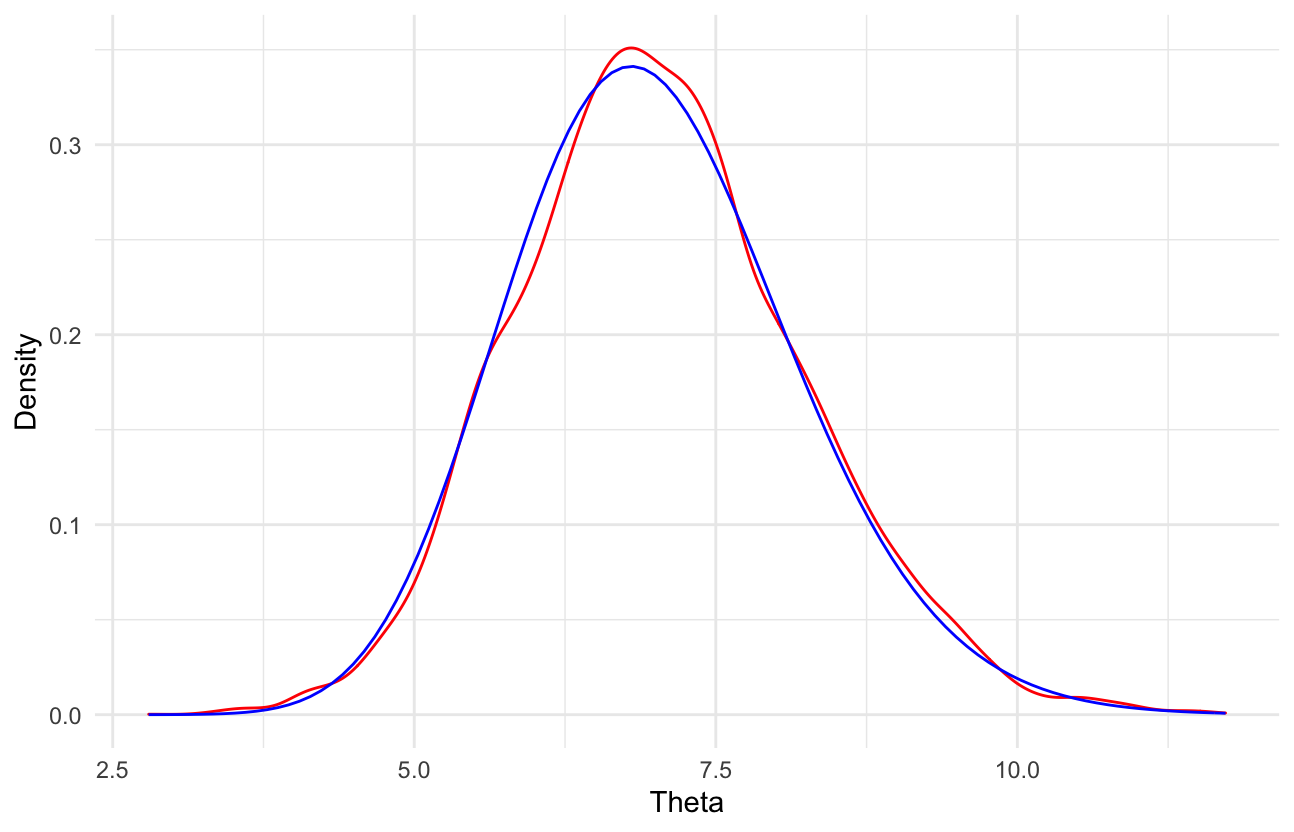
\includegraphics[width=100mm,scale=0.5]{Figure1.png}
        \caption{Simulated Posterior Distribution from Metropolis-Hastings (Red Line) versus True Posterior Distribution (Blue Line)}
        \label{fig:my_label}
    \end{figure}
    Upon completing more algebra, we find the normalized density function is that of a $\text{GAMMA} \left( \sum_{i} y_{i} + \alpha, n + \beta \right)$ distribution. The density function for this distribution (with some parameters given) is shown (blue line) in figure 1.
    \\[1\baselineskip]
    We can see from Figure 1 how our sample distribution approaches the desired posterior distribution over large-scale simulation. This means that we are able to sample from many unknown posterior distributions, despite not being able to solve their normalizing constant.
\end{example}
\section{Gibbs Sampler}
The Gibbs Sampler is a particular case of the Metropolis-Hastings Algorithm. It applies the algorithm in partial, fully conditional steps. Often, we have access to conditional distributions, and limited access to joint distributions for a vector of parameters. For our purposes, we will consider the case where $\boldsymbol{\Theta} = \left( \Theta_{1}, \Theta_{2} \right)'$, but it can be extended for more variables.

\pagebreak
\noindent
The steps for the Gibbs Sampler are as follows:
\begin{enumerate}
    \item Set $\theta_{2}$ to any estimate
    \item Select $\theta_{1}^{*} \sim f \left( \theta_{1}^{*} | \theta_{2}, x \right)$
    \item Select $\theta_{2}^{*} \sim f \left( \theta_{2}^{*} | \theta_{1}^{*}, x \right)$
    \item $\left( \theta_{1}^{*}, \theta_{2}^{*} \right)$ is a draw from the joint distribution. Repeat from step 2.
\end{enumerate}
For this process, the transition kernel can be considered:
\begin{align*}
    K \left( \theta_{1}, \theta_{2} | \theta_{1}^{*}, \theta_{2}^{*}  \right) &= f_{\Theta_{1} | \Theta_{2}} \left( \theta_{1}^{*} | \theta_{2}\right) f_{\Theta_{2} | \Theta_{1}} \left( \theta_{2}^{*} | \theta_{1}^{*} \right)
\end{align*}
Where $f_{\Theta_{1} | \Theta_{2}}$ is the conditional density of $\Theta_{1} | \Theta_{2}$, and $f_{\Theta_{2} | \Theta_{1}}$ is the conditional density of $\Theta_{2} | \Theta_{1}$. 
\begin{theorem}
    The joint distribution of $\Theta_{1}$ and $\Theta_{2}$, $f_{\Theta_{1}, \Theta_{2}} \left( \theta_{1} , \theta_{2}\right)$ is the stationary distribution of $K$.
\end{theorem}
\noindent
\textit{Proof:}
\begin{align*}
    \left( Kf_{\Theta_{1}, \Theta_{2}} \right) \left( \theta_{1}^{*}, \theta_{2}^{*} \right) &= \int \int f_{\Theta_{1}, \Theta_{2}} \left( \theta_{1}, \theta_{2} \right) K \left( \theta_{1}, \theta_{2} | \theta_{1}^{*}, \theta_{2}^{*}  \right) d \theta_{1} d \theta_{2} \\[1em]
    &= \int \int f_{\Theta_{1}, \Theta_{2}} \left( \theta_{1}, \theta_{2} \right) f_{\Theta_{1} | \Theta_{2}} \left( \theta_{1}^{*} | \theta_{2}\right) f_{\Theta_{2} | \Theta_{1}} \left( \theta_{2}^{*} | \theta_{1}^{*} \right) d \theta_{1} d \theta_{2} \\[1em]
    &= \int \int f_{\Theta_{1}, \Theta_{2}} \left( \theta_{1}, \theta_{2} \right) \frac{f_{\Theta_{1}, \Theta_{2}} \left( \theta_{1}^{*} , \theta_{2}\right)}{f_{\Theta_{2}} \left( \theta_{2} \right)} \frac{f_{\Theta_{1}, \Theta_{2}} \left( \theta_{1}^{*} , \theta_{2}^{*} \right)}{f_{\Theta_{1}} \left( \theta_{1}^{*} \right)} d \theta_{1} d \theta_{2} \\[1em]
    &= \int f_{\Theta_{2}} \left(\theta_{2} \right) \frac{f_{\Theta_{1}, \Theta_{2}} \left( \theta_{1}^{*} , \theta_{2}\right)}{f_{\Theta_{2}} \left( \theta_{2} \right)} \frac{f_{\Theta_{1}, \Theta_{2}} \left( \theta_{1}^{*} , \theta_{2}^{*} \right)}{f_{\Theta_{1}} \left( \theta_{1}^{*} \right)} d \theta_{2} \\[1em]
    &= \int f_{\Theta_{1}, \Theta_{2}} \left( \theta_{1}^{*} , \theta_{2}\right) \frac{f_{\Theta_{1}, \Theta_{2}} \left( \theta_{1}^{*} , \theta_{2}^{*} \right)}{f_{\Theta_{1}} \left( \theta_{1}^{*} \right)} d \theta_{2} \\[1em]
    &= f_{\Theta_{1}} \left( \theta_{1}^{*} \right) \frac{f_{\Theta_{1}, \Theta_{2}} \left( \theta_{1}^{*} , \theta_{2}^{*} \right)}{f_{\Theta_{1}} \left( \theta_{1}^{*} \right)} \\[1em]
    &= f_{\Theta_{1}, \Theta_{2}} \left( \theta_{1}^{*} , \theta_{2}^{*} \right) \; \; \; \; \; \Box
\end{align*} 
Therefore, we can use the Gibbs Sampler method to sample from any joint distribution given conditional distributions.
\\[1\baselineskip]
\begin{example}
    Suppose that we want to draw samples from the multivariate normal distribution below:
    \begin{align*}
        \left( \theta_{1}, \theta_{2} \right)' &\sim \text{N} \left(
        \begin{pmatrix} 2 \\
                        3 \end{pmatrix}, 
        \begin{pmatrix} 7 & 2 \\
                        2 & 10 \\ \end{pmatrix} \right)
    \end{align*}
    The conditionals from this density function are given by:
    \begin{align*}
        \theta_{1} | \theta_{2} &\sim N \left( 2 + \frac{1}{5} \left( \theta_{2} - 3 \right), \frac{33}{5} \right) \text{, and} \\[1em]
        \theta_{2} | \theta_{1} &\sim N \left( 3 + \frac{1}{5} \left( \theta_{1} - 2 \right), \frac{66}{7} \right)
    \end{align*}
    \noindent
    Using the steps we developed for performing a Gibbs Sampler, we started with $\theta_{2} = 3$, and repeated steps 2-4 11,000 times, retaining the last 10,000 iterations. The resultant simulated density is shown in Figure 2.
\end{example}

\begin{figure}
    \centering
    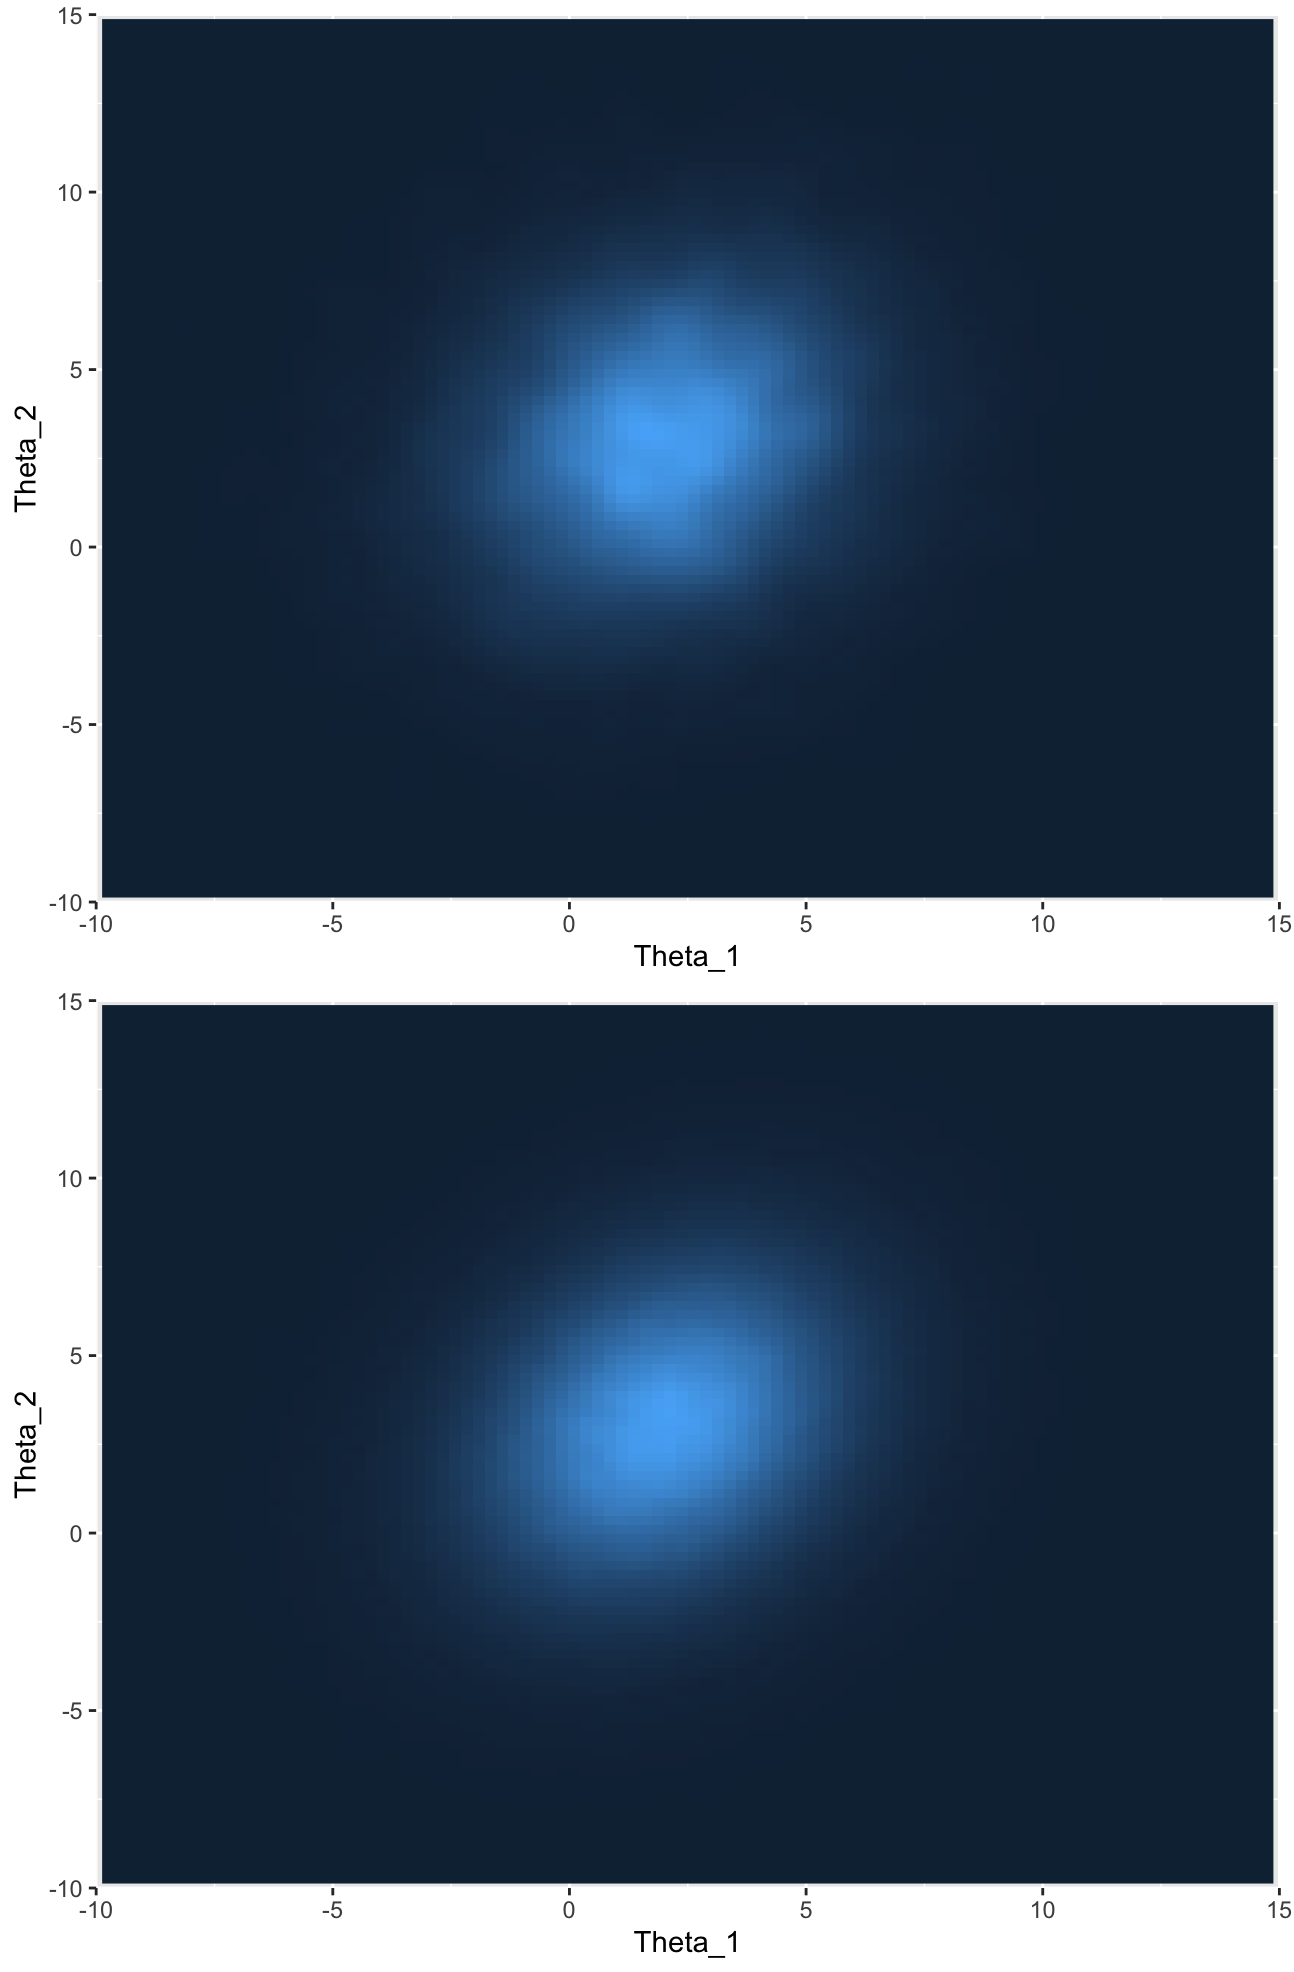
\includegraphics[width=75mm,scale=0.5]{Figure2.png}
    \caption{Heatmap of the Simulated Mulitvariate Normal Density from Example 3 (Top) versus True Multivariate Normal Density (Bottom).} 
    \label{fig:my_label}
\end{figure}

\section{Research Directions}
At the current time, the field of machine learning is using Markov Chain Monte Carlo to assist the field of AI. It allows researchers to draw samples from density functions which are impossible to solve for. Current research involves finding efficient proposal kernels to improve computational speed of various algorithms. Ziheng Yang and Carlos E. Rodríguez \cite{ziheng} propose a unique class of Bactrian kernels which claim to be 50\% more efficient than the usual Gaussian proposal kernel. The idea behind the Bactrian kernels is to create a mixture distribution from multiple component distributions to increase efficiency. A selection of these distributions are shown in Figure 3.

\begin{figure}[h]
    \centering
    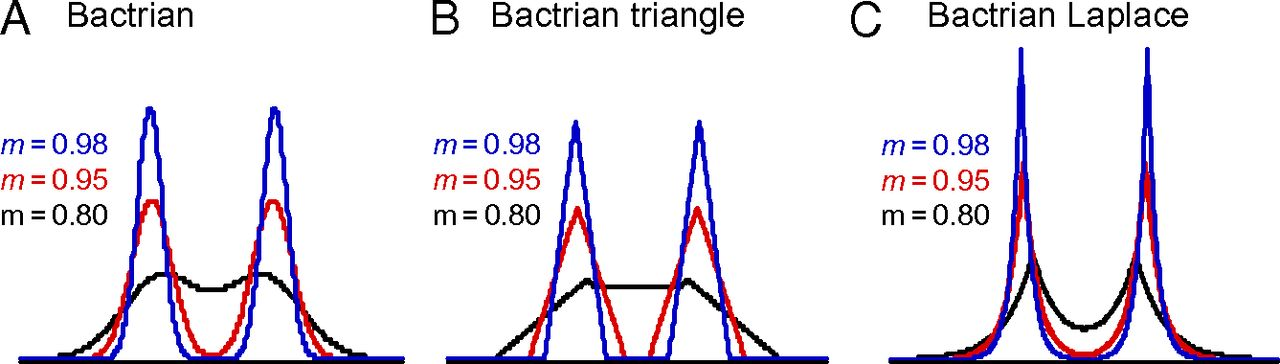
\includegraphics[width=100mm,scale=0.5]{Figure3.jpeg}
    \caption{Some Bactrian Proposal Distributions given by Yang and Rodríguez (2013)} 
    \label{fig:my_label}
\end{figure}

\noindent
Another more recent development in Markov Chain Monte Carlo comes from Matthew Hoffman, Alexey Radul, and Pavel Sountsov \cite{hoff} in their use of no-U-turn sampler (NUTS) which eliminates the simulation length requirement parameter which can limit the capabilities of other simulations discussed when working with high-dimensional distributions. Instead of the random walk idea used by the Metropolis-Hastings algorithm, NUTS uses a recursive algorithm which builds a set of likely candidate points, and aborts when it starts doubling back on itself. With machine learning heading in a direction of such high-dimensional models, simulations which cut down their simulation time are extremely important.
\\[1\baselineskip]
\noindent
With Markov Chain Monte Carlo being so prevalent in modern statistics, it is important to understand both the theory and applications before going into the field.
\pagebreak
\section{Questions (+ Answers)}
\begin{enumerate}
    \item Show that the Kernel $P_{mh}$ from Theorem 2 is reversible with respect to the distribution with unnormalized density function $g$ in the case where $r \left( x, y \right) < 1$.
    \\[1\baselineskip]
    \textit{Solution.} By our assumption, it must be that $a \left( y, x \right) = 1$ and $a \left( x, y \right) = r \left( x, y \right)$. Now, we can take:
    \begin{align*}
    \int \int f \left( x, y \right) g \left( x \right) q \left( x, y \right) a \left( x, y \right) \mu \left( dx \right) \mu \left( dy \right) &= \int \int f \left( x, y \right) g \left( x \right) q \left( x, y \right) r \left( x,y \right) \mu \left( dx \right) \mu \left( dy \right) \\[1em]
    &= \int \int f \left( x, y \right) g \left( x \right) q \left( x, y \right) \frac{g \left( y \right) q \left( y, x \right)}{g \left( x \right) q \left( x, y \right)} \mu \left( dx \right) \mu \left( dy \right) \\[1em]
    &= \int \int f \left( x, y \right) g \left( y \right) q \left( y, x \right)  \mu \left( dx \right) \mu \left( dy \right) \\[1em]
    &= \int \int f \left( x, y \right) g \left( y \right) q \left( y, x \right) a \left( y, x \right) \mu \left( dx \right) \mu \left( dy \right)
    \end{align*}
    The last equality implies that the order of $x, y$ are irrelevant in this case, so we can continue as we did in Theorem 2, and obtain the same proof.

    \item Reproduce the chart given in Example 1 for $\alpha = \beta = 2$, $\mathbf{y} = \left( 10, 10, 13 \right)'$, for $11,000$ iterations where the first $1,000$ iterations are removed.
    \\[1\baselineskip]
    \textit{Solution.} See attached code.
\end{enumerate}



% add your main body sections here

% open questions section
% !TEX root = ../main.tex

% open questions section

\section{Open questions and research directions}

%%%% appendix
\clearpage
\appendix

% exercises and problems
% !TEX root = ../main.tex

% Exercises section

\section{Exercises}

% any other appendix sections


% bibliography
\printbibliography

\end{document}
